\begin{inhalt}
\renewcommand*\chapterpagestyle{scrheadings}
\chapter{Ergebnisse \& Ausblick}

Die in Kapitel \ref{sec:PCBVersion2} entwickelte Platine konnte erfolgreich entworfen und bestückt werden (Abb. \ref{fig:fertigeplatine}). Sie wurde erfolgreich auf ihre Funktionalität getestet.

\bigskip \\

Der Mikrocontroller liest die Messdaten der Sensoren erfolgreich aus und gibt sie auf dem Display aus (Abb. \ref{fig:fertigesGerat}). Das Display besitzt, wie in Kapitel \ref{sec:display interface} beschrieben, drei verschiedene Seiten, zwischen denen gewechselt werden kann. Die Taster erfüllen dabei ihre Funktionen (Kapitel \ref{sec:BeutzerInteraktionen}). Die Datenübertragung an den Webserver über HTTPS, sowie die Skala am Display, ist mit Stand vom 02.04.2025 aufgrund von Zeitknappheit noch nicht funktionstüchtig.


\begin{figure}[!htb]
    \centering
    \begin{subfigure}[b]{0.49\textwidth}
        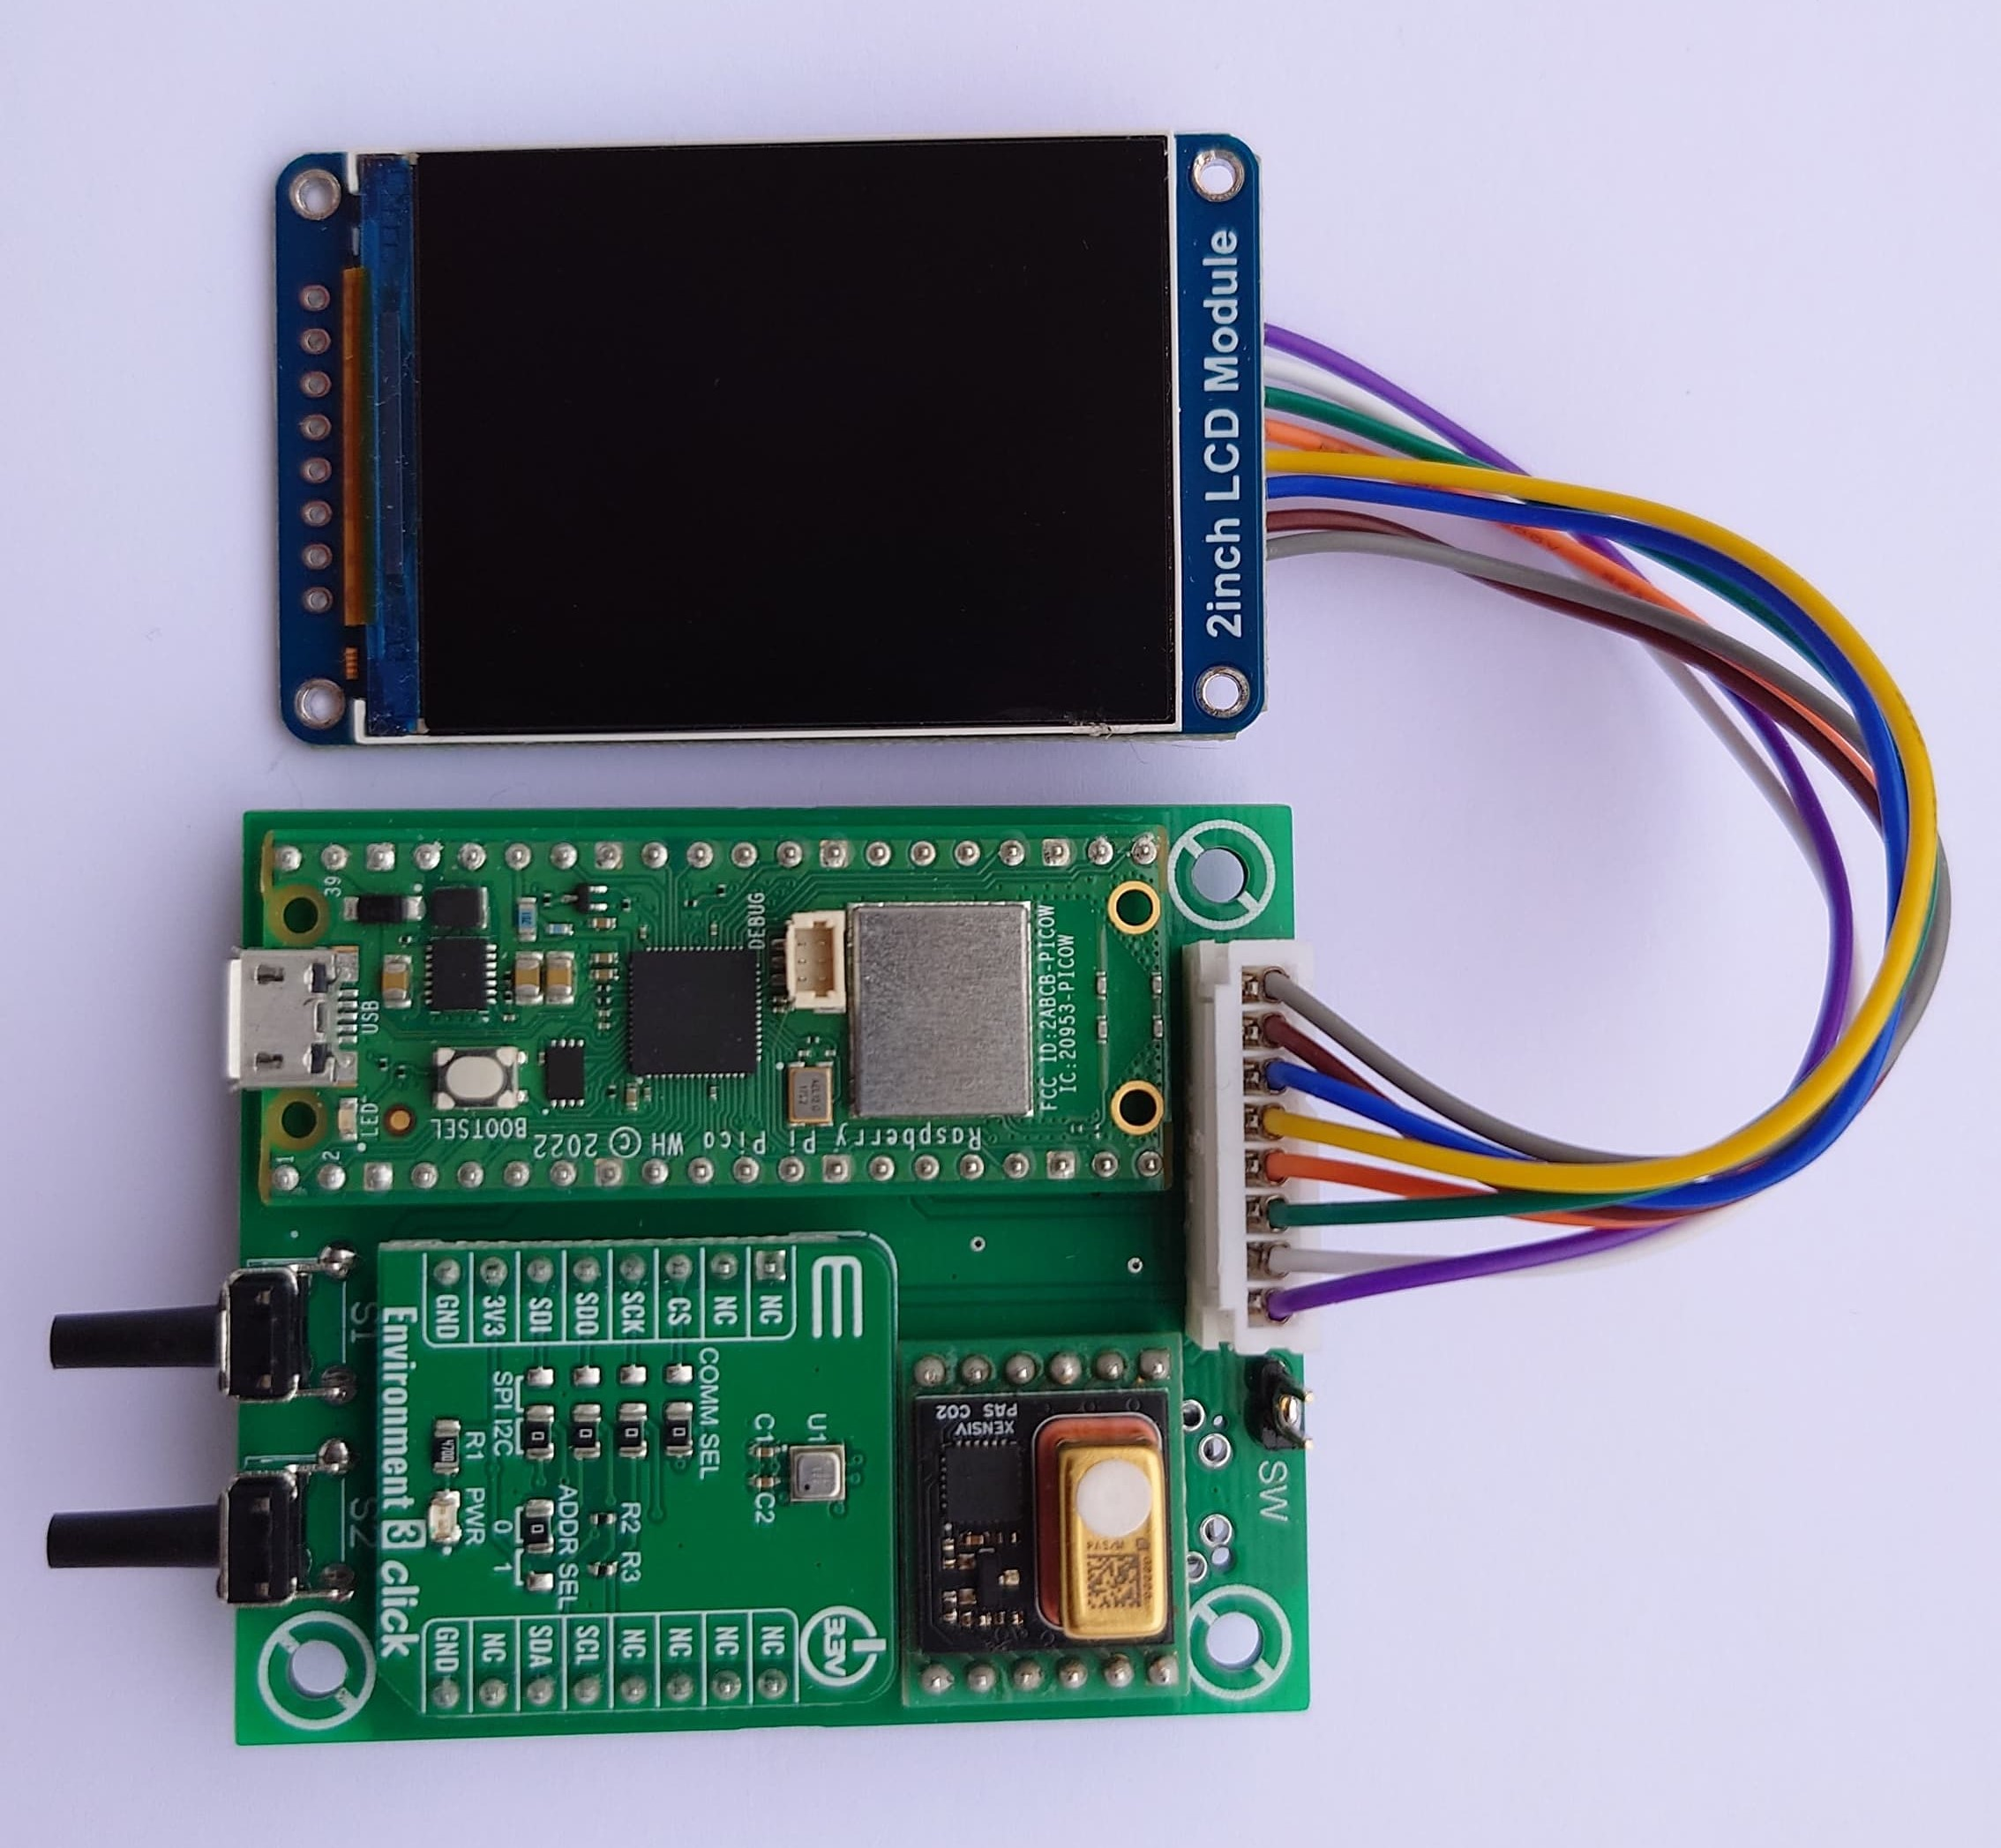
\includegraphics[width=\textwidth]{files/Tobias/pics/Platine (2).jpg}
        \caption{Fertiggestellte Platine}
        \label{fig:fertigeplatine}
    \end{subfigure}
    \hfill
    \begin{subfigure}[b]{0.49\textwidth}
        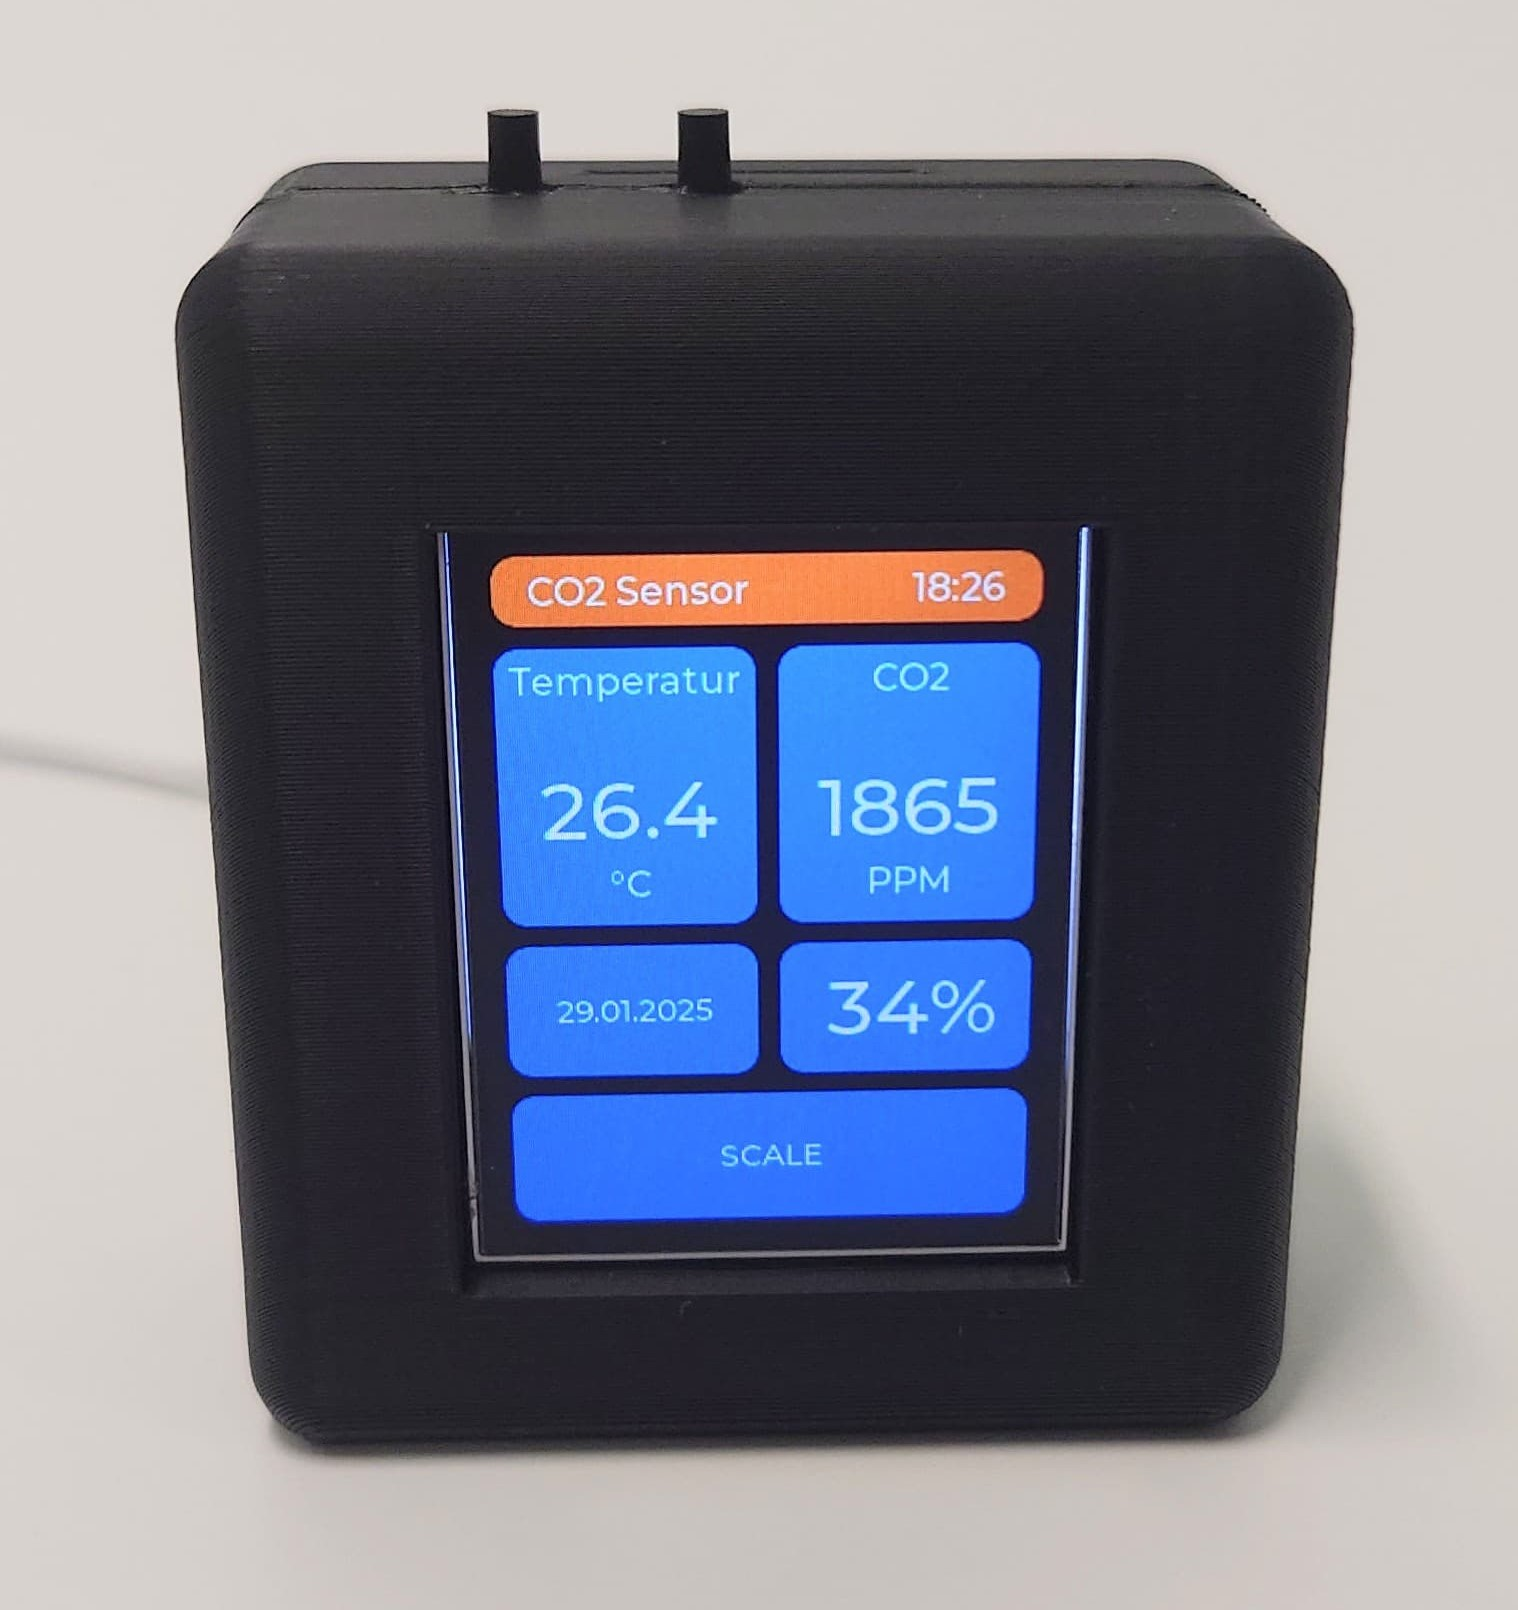
\includegraphics[width=\textwidth]{files/Tobias/pics/Geraet.jpg}
        \caption{Fertiggestelltes Messgerät}
        \label{fig:fertigesGerat}
    \end{subfigure}
    \caption[Hardware \& Mikocontrollerprogrammierung - Ergebnisse]{Hardware \& Mikocontrollerprogrammierung - Ergebnisse}
    \label{fig:Ergebnisse}
\end{figure}


Die ursprünglich geplante App wurde verworfen, da sich nach intensiver Recherche \cite{youtube_no_app} herausstellte, dass sich die Software besser als Web-Anwendung anstatt als mobile Smartphone-App umsetzen lässt.  
Aus diesem Grund wurden alle zu Beginn erstellten Flutter-Projekte pausiert und stattdessen eine Webseite entwickelt.  
Die in Kapitel \ref{ref:Website} vorgestellte Webseite konnte erfolgreich fertiggestellt werden.  
Zwar sind aktuell noch einige kleinere Bugs vorhanden, diese sollen jedoch in Zukunft behoben werden.  
Die Realtime-Funktionalität, beispielsweise in den Diagrammen, funktioniert bereits zuverlässig.
\vspace{0.1cm}
Das Gehäuse funktioniert einwandfrei, es konnten keine Fehler festgestellt werden und es wurde erfolgreich und zuverlässig getestet.


\begin{figure}[!htb]
    \centering
    \begin{subfigure}[b]{0.49\textwidth}
        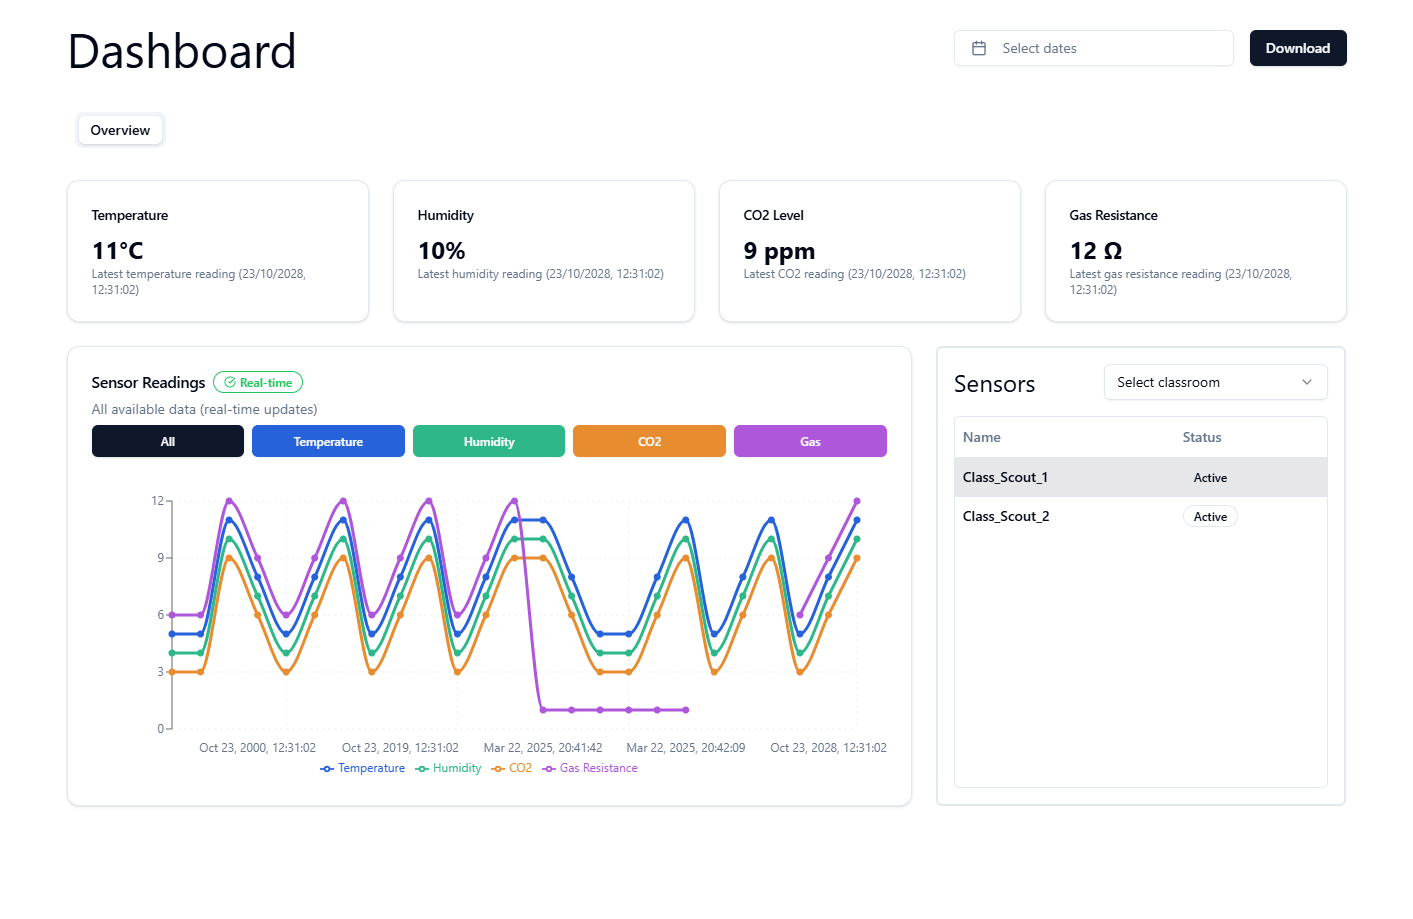
\includegraphics[width=\textwidth]{files/Thomas/pics/Website/dashbord/dashbaord-screen.png}
        \caption{Fertiges Dashboard}
        \label{fig:dashboard_fertig}
    \end{subfigure}
    \hfill
    \begin{subfigure}[b]{0.49\textwidth}
        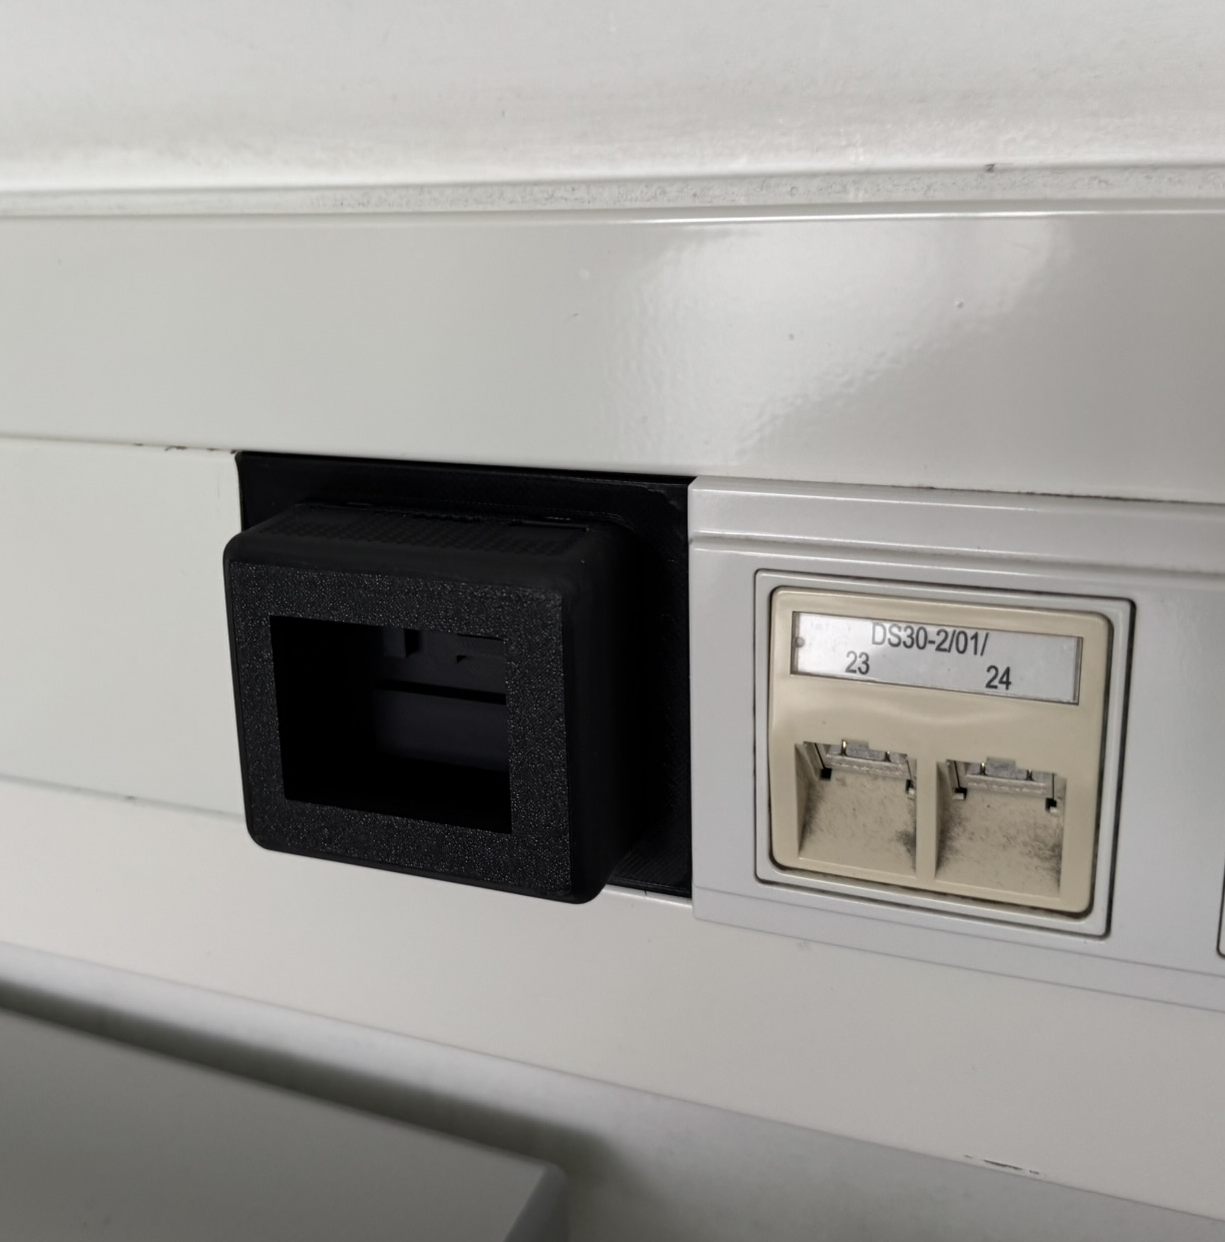
\includegraphics[width=\textwidth]{files/Thomas/pics/image.png}
        \caption{Fertiges Gehäuse in Kabelkanal}
        \label{fig:dashboard_zweites}
    \end{subfigure}
    \caption[Fertige Diplomarbeitsteile]{Fertiges Diplomarbeitsteile}
    \label{fig:dashboard_vergleich}
\end{figure}


Für die weitere Entwicklung wurde erkannt, dass sich das globale State-Management einfacher mit Cookies als über die URL realisieren lässt.  
Hierfür könnten Bibliotheken wie \texttt{zustand} verstärkt zum Einsatz kommen, da \texttt{Next.js} im Gegensatz zu anderen JavaScript-Frameworks kein eingebautes globales State-Management bietet.  
Außerdem wäre es sinnvoll, künftig auch den Status der Sensoren in die Webseite zu integrieren.





\end{inhalt}